% This is LLNCS.DEM the demonstration file of
% the LaTeX macro package from Springer-Verlag
% for Lecture Notes in Computer Science,
% version 2.4 for LaTeX2e as of 16. April 2010
%
\documentclass{llncs}
\usepackage{pdflscape}
\usepackage{amsfonts}
\usepackage{amsmath}
\usepackage{tikz}
\usetikzlibrary{arrows,positioning}
\usepackage{rotating}



% Custom Macros
\newcommand{\figref}[1]{{Figure}~\ref{#1}}
\newcommand{\tabref}[1]{{Table}~\ref{#1}}
\newcommand{\secref}[1]{{Section}~\ref{#1}}
\newcommand{\appref}[1]{{Appendix}~\ref{#1}}

\hyphenation{MIRACL}

\newcommand{\K}{\ensuremath{\mathtt{s}}}
\newcommand{\msg}{\ensuremath{\mathtt{m}}}
\newcommand{\ms}{\ensuremath{ms}}
\newcommand{\id}[1]{\ensuremath{\mathtt{id}_{#1}}}


\begin{document}

\title{Practical Identity Based Broadcast Encryption for Online Social Networks}

% \author{}
\author{Filipe Beato \and Stijn Meul \and Bart Preneel}
\institute{ESAT/COSIC - KU Leuven and iMinds\\ Leuven, Belgium\\
\email{\{first.lastname\}@esat.kuleuven.be}}

\maketitle   % typeset the title of the contribution

\begin{abstract} Nowadays Online Social Networks (OSNs) constitute an important and useful communication channel. At the same time, coarse-grained privacy preferences protect the shared information insufficiently. Cryptographic techniques can provide interesting mechanism to protect privacy of users in OSNs. However, this approach faces several issues, such as, OSN provider acceptance, user adoption, key management and usability. We suggest a practical solution that uses Identity Based Encryption (IBE) to simplify key management and enforce confidentiality of data in OSNs. Moreover, we devise an outsider anonymous broadcast IBE scheme to disseminate information among multiple users, even if they are not using the system. Finally, we demonstrate the viability and tolerable overhead of our solution via an open-source prototype.
\end{abstract}


\section{Introduction}

Online Social Networks (OSNs), such as Facebook, Google+, and Twitter are increasingly being used and have become a prominent communication channel for many millions of users. OSNs offer users an efficient and reliable channel to distribute and share information. At the same time, OSNs store large amounts of data which prompts several privacy concerns. In particular, it is possible to infer a considerable amount of sensitive information from the shared and stored content. Currently, users are allowed to configure ``privacy preferences'' in order to limit and select which users or groups can access the shared content. These preferences are generally too coarse-grained and difficult to configure~\cite{bonneau2010privacy}. Another problem is that these preferences do not exclude the provider along with the dangers of data leaks~\cite{fischetti11hacker} nor external governments~\cite{prism}.

All these worrisome issues motivate the need for effective techniques to properly protect user's privacy in OSNs. Several solutions have been proposed and advocated to use cryptographic mechanisms in order to address the privacy issues, either by an add-on atop of existing OSNs~\cite{BadenPersona,BeatoScramble,Guha:2008,Luo:2009}, or by complete new privacy-friendly architectures~\cite{DBLP:conf/sp/CristofaroSTW12}, mainly decentralized~\cite{DBLP:conf/wowmom/CutilloMO11,NYT2010.Diaspora}. In general, those solutions suffer from user adoption and key management issues as users are required to register and then share, certify and store public keys~\cite{article2400}. Completely new architectures represent a difficult step for users as the trade off of moving away from the commonly used social ecosystem compared with the risk of losing interactions is high. Arguably, current centralized OSNs are here to stay and will be continue to be actively used by millions of people. In light of recent events, such as Edward Snowden's whistle-blowing on US surveillance programs~\cite{prism}, OSN providers have all interest to maintain their users and a privacy-friendly image. Hence, it is important to protect user's sharing information and the recipient set as it can contain private and sensitive information to the user. 


\paragraph{Main Idea:}

Identity Based Encryption (IBE)~\cite{DBLP:conf/crypto/Shamir84} solutions overcome the key management problem as the public key of the user can be represented by any valid string, such as the email, unique \id{}\ and username. Therefore, by using a OSN username any savvy and concerned user can share encrypted content with other users who are not using the solution, thereby motivating curious ones to use the system as well. Nevertheless, IBE-based systems require a trusted central Private Key Generator (PKG) server to generate the private parameters for each user based on a master secret. Consequently, such an architecture only shifts the trusted party from the OSN to the PKG. However, this problem can be mitigated if the master secret is divided among multiple PKGs following a Distributed Key Generation (DKG)~\cite{Pedersen:1991:NIS:646756.705507} protocol based on Verifiable Secret Sharing (VSS)~\cite{DBLP:conf/focs/ChorGMA85}. A DKG protocol allows $n$ entities to jointly generate a secret requiring that a threshold $t$ of the $n$ entities does not get compromised. In fact, each entity holds only a share of the master secret, that can be reconstructed by at least $t$ shares. 

Many OSN users are not only represented on a single OSN but on several, thus, can also hold multiple public keys. Moreover, the multi-PKG setting could be supported and maintained by several existing OSNs. In particular, collaboration between OSN providers that compete along is assumed to be a difficult task and orthogonal to their economical business model. 
\figref{fig:overview} depicts an overview example of the proposed model, where a user authenticates to $t$-PKGs of his choice using, e.g., a similar token as in open id protocols, to retrieve his private key. This action can be performed after the reception of encrypted content as a consequence of user curiosity .
The PKG servers can also be represented by governmental entities from different continents, with no incentives to collaborate nor overcome more powerful adversaries using legal measures~\cite{facebook-subpoena} among at least $t$-PKGs. 

% -----------------------------------------------------------------------------
\begin{figure}[ht]
    \begin{center}
    \scalebox{0.78}{
        \begin{tikzpicture}[auto, node distance=1mm,
            block/.style={rectangle,text width=6em,text centered,minimum height=11mm},
            line/.style={draw,very thick, ->},
            line2/.style={draw,very thick, <->},
            leg/.style={font=\scriptsize,text centered},
            ]
            % \draw[help lines] (-6,-5) grid (8,3);
            \draw[dashed] (-5,6) -- (5,6) -- (5,3) -- (-5,3) -- (-5,6);
            \path
                % title of PKG BOX
                (0, 6.5) node {\textbf{Pool of Multiple PKGs}}
                
                % Bottom part
                (-5.5,0) node [block] (user) {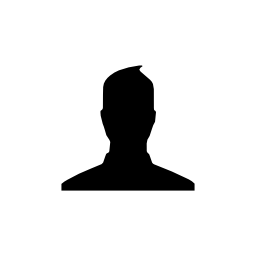
\includegraphics[scale=0.2]{images/fbuser.png}}
                (0,0) node [block] (fb) {
\includegraphics[scale=0.12]{images/fb_icon.png}}
                (5.5, 0) node [block] (friends) {
\includegraphics[scale=0.3]{images/fbfriends.png}}

                %Top part (PKG lists)
                (-3,4) node [block] (linkedin) {
\includegraphics[scale=0.1]{images/linkedin.png}}
                (-4,5) node [block] (fbpkg) {
\includegraphics[scale=0.06]{images/fb_icon.png}}
                (1.2,5) node [block] (gplus) {
\includegraphics[scale=0.08]{images/gplus.png}}
                (-2,5.2) node [block] (tumblr) {
\includegraphics[scale=0.1]{images/tumblr.png}}
                (2.8,4) node [block] (pin) {
\includegraphics[scale=0.05]{images/pinterest.png}}
                (4.2,5) node [block] (tor) {
\includegraphics[scale=0.1]{images/tor.png}}
                (-0.5,4) node [block] (twitter) {
\includegraphics[scale=0.05]{images/twitter.png}};

            \node[below=of fb] {\textbf{Facebook}};
            \node[below=of user] {\textbf{User}};
            \node[below=of friends] (frdcaption) {\textbf{Subset of Recipients}};
            \node[below=of frdcaption] {\textbf{s.t., $\mathcal{S}=\{\id{1},\id{2},\ldots,\id{\eta}\}$}};


            \begin{scope}[every path/.style=line]
                \path (user.east) -- (fb.west);               
            \end{scope}   

            % Legend
            \path (-2.8,0.35) node [leg] {Publish: $C\leftarrow$ Encrypt(\msg,$\mathcal{S}$)};
            \path (2.7,0.35) node [leg] {Retrieve $C$};
            \node[right=of friends] {Decrypt($C$)};
                
            \begin{scope}[every path/.style=line2]
                \path (fb) -- (friends);
                \path[dashed] (friends.north) -- (tor.south);
                \path[dashed] (5.1,1) -- (3.1,3.4);
                \path[dashed] (4.7,0.95) -- (0.5,3.5);
            \end{scope}
        \end{tikzpicture}
    }
    \end{center}
    \caption{Multiple $(n,t)$-PKG IBE for OSNs overview, for a message \msg\ published for the set $\mathcal{S}$ for $t=3$.}
    \label{fig:overview}
\end{figure}
% -----------------------------------------------------------------------------

% \begin{itemize}
%     \item Motivate the Multiple servers, e.g., assumptions that business model does not allow , and example open id. Also that requires at least t compromised PKGs to possible get the key -> point that this is hard
%     \item motivate new strategy that users can encrypt to other users even if the others don't run the system YET.
%     \item mention that efficiency for average users.
%     \item extension to scramble implementation, encryption is stored in servers and the link to the OSN
%     \item highlight that the key needs to be updated only once every month (for instance)
%     \item using VSS users can verify if the shares are valid ones and detect possible malicious PKGs and then announce
% \end{itemize}

\paragraph{Contribution:} In this paper, we propose a novel practical solution that uses IBE with multiple untrusted PKGs atop of current OSNs. 
We highlight the fact that those multi-PKGs can be supported by several existing OSNs under the business competition assumption, and motivated by the possible attractive incentives towards more privacy concerned audience. 
Along with the multi-PKG IBE model we devise an IBE broadcast encryption protocol to support multiple recipients. Using a broadcast IBE-based mechanism we allow users to share content with multiple recipients, even if they are not using the system, and, thus, enforce confidentiality of the data while hiding the recipient set. Finally, we implemented our solution on top of the Scramble Firefox extension~\cite{BeatoScramble}, and show that only a small overhead is required.
 
\paragraph{Roadmap:} The remainder of this paper is organized as follows. \secref{sec:background} gives a brief overview of the cryptographic background. Next, \secref{sec:model} presents the model followed by the description of the suggested solution in \secref{sec:solution}. \secref{sec:impl} describes the implementation details, while \secref{sec:relwork} reviews related work. Finally, \secref{sec:conc} summarizes and concludes the paper.






\section{Background}\label{sec:background}
In this section we briefly overview the cryptographic tools and building blocks used in this paper. For ease of explanation we omit the definitions of the underlying cryptographic primitives. This section 
can, however, be skipped with no loss of continuity.

\subsection{Identity Based Encryption}
The concept of Identity Based Encryption (IBE) was introduced by Shamir~\cite{DBLP:conf/crypto/Shamir84}, with the main idea of using any string as the public key. IBE requires no certificates as users can rely on publicly known identifiers such as an e-mail address or a telephone number, thus, reducing the complexity of establishing and managing a public key infrastructure. Boneh and Franklin propose the first practical IBE using bilinear pairings \cite{BonehFranklinIBE}, later extended by Gentry~\cite{GentryRandomOracles}. 

A generic IBE scheme is composed of four randomized algorithms:
\begin{description}
    \item[\texttt{IBE.Setup:}] On the input of a security parameter $\lambda$, outputs a master secret $s$ and the master public parameters $params$. 
    \item[\texttt{IBE.Extract:}] Takes the public parameters $params$, the master secret $s$, and an \id{} and returns the private key $d_{\id{}}$.
    \item[\texttt{IBE.Encrypt:}] Returns the encryption $C$ of the message \msg\ on the input of the $params$, the \id{}, and the arbitrary length message \msg. 
    \item[\texttt{IBE.Decrypt:}] Reconstruct \msg from $C$ by using the secret $d_{\id{}}$.
\end{description}

The \texttt{IBE.Setup} and \texttt{IBE.Extract} algorithms are executed by a trusted Private Key Generator (PKG) server, whereas \texttt{IBE.Encrypt} and \texttt{IBE.Decrypt} are performed by two players, e.g., Alice and Bob. Consequently, key escrow is performed implicitly in the classic IBE scheme as the PKG holds the master secret key.

\subsection{Anonymous Broadcast Encryption}
Broadcast encryption (BE) was introduced by Fiat and Naor~\cite{FiatBE}, as a public-key generalization to a multi user setting. A BE scheme allows a user to encrypt a message to a subset $\mathcal{S}$ of users, such that, only the users in the set $\mathcal{S}$ are able to decrypt the message. The computational overhead of the BE is generally bound to the ciphertext and the number of recipients. To overcome this issue, the set $\mathcal{S}$ of recipients is generally known. Barth et al.~\cite{BarthBonehWaters} and Libert et al.~\cite{LibertANOBE} extended the notion of BE and introduced the notion of Anonymous Broadcast Encryption (ANOBE) scheme, where the recipient set $\mathcal{S}$ remains private even to the members in the set. Fazio and Perera~\cite{FazioOutsiderANOBE} suggested the notion of outsider anonymous BE that represents a more relaxed notion of ANOBE.  

A generic BE and ANOBE scheme consists of four randomized algorithms:
\begin{description}
    \item[\texttt{BE.Setup:}] On the input of a security parameter $\lambda$, generates the public parameters $params$ of the system.
    \item[\texttt{BE.KeyGen:}] Returns the public and private key ($pk,sk$) for each user according to the $params$.
    \item[\texttt{BE.Encrypt:}] Takes the set $\mathcal{S}=\{pk_i \ldots pk_{|\mathcal{S}|}\}$ along with the secret message \msg\ and generates $C$.
    \item[\texttt{BE.Decrypt:}] Reconstructs \msg\ from $C$ using the private key $sk_i$ if the corresponding public key $pk_i \in \mathcal{S}$. Otherwise, return $\bot$.
\end{description}

Note that the $pk$ can be represented by the \id{} value from the IBE scheme. 


\subsection{Distributed Key Generation}
Distributed Key Generation (DKG) was introduced by Pedersen~\cite{Pedersen:1991:NIS:646756.705507} to allow a group of entities to collaboratively setup a secret sharing environment over a public channel.
Secret sharing was introduced by Shamir~\cite{Shamir1979} and consists of dividing a secret \K\ into $n$ shares among $n$ entities, such that, only a subset of size greater than or equal to a threshold $t$ can reconstruct \K, where $t \geq n$. In practice, a random secret \K\ is generated along with a polynomial $f(x)$ of degree $t-1$ such that $f(0)=\K$, where the shares $s_i$ are represented by different points on the polynomial. Any entity with $t$ or more shares can reconstruct $f(x)$ using Lagrange interpolation, and subsequently find $\K$. Further, Chor et al.~\cite{DBLP:conf/focs/ChorGMA85} suggested a Verifiable Secret Sharing (VSS) scheme to allow anyone to verify that the right shares are used. The scheme was extended by Feldman~\cite{Feldman:1987:PSN:1382440.1383000} and Pedersen~\cite{Pedersen:1991:NIS:646756.705507}. 

For multiple parties to jointly generate a secret sharing \K, all entities are required to participate in a DKG scheme. Each entity $i$ involved generates a different $\K_i$ and $f^i(x)$, and later on distributes and verifies the shares $s_{ij}$. Hence, a generic DKG does not require a trusted party, as the master secret is computed as the sum of all the polynomials and can only be retrieved by joining $t$ shares. A generic DKG protocol consists of two phases:

\begin{description}
    \item[\texttt{DKG.Setup:}] Every entity $i$ generates a random secret $\K_i$ and computes a polynomial of degree $t-1$. The entity $i$ Distributes a valid share $s_{ij}$ over all the other $j$ entities, along with the commitment to the share. Each entity $j$ verifies the shares and computes the new share $s_j = \sum_i s_{ij}$. The master secret is unknown by each party, and composed by the origin point on the sum of all polynomials $f^i(x)$.
    \item[\texttt{DKG.Reconstruct:}] Each entity $i$ broadcasts its share $s_i$, and with $t \leq n$ shares, one can reconstruct the master secret $s$.
\end{description}

The DKG protocol is secure assuming that no adversary is able to corrupt $t$ parties or more. 


\section{Model}\label{sec:model}
We consider that a user $u$ to be a member of an OSN, such as Facebook, Twitter or Google+. Such $u$ is connected with other users in the same OSN by a friendship relation with who shares information~\cite{boyd2008social}. Inherently, $u$ aims to interact and share information \msg\ with other users. Each user holds a public and private key pair which is given by an IBE identity server (composed of multiple PKG servers), such that the public key is represented by the \id{} of the user in the OSN. Note that each user can be registered into multiple OSNs and hold different public keys and \id{}s. We assume that the authentication between the user and the identity servers is done using a token similarly to open id, and performed under an authenticated channel, e.g., TLS.

% Don't we want users to be able to discuss on updates of common friends without the need for these users to be a connection on the OSN?

\paragraph{Threat Model:}
We consider an adversary to be any entity attempting to passively access the shared information \msg\ by monitoring the sharing channel but with no motivational incentive to tamper with the content. This can be any curious user in the OSN, the OSN provider or even a government agency~\cite{prism}. Such an adversary should not learn the content nor the identity of the members in the recipient set $\mathcal{S}$, otherwise we consider that the adversary breaks confidentiality and the outsider recipient anonymity of the protocol as defined in~\cite{FazioOutsiderANOBE}.
In addition, we assume that such an adversary cannot compromise more than $t$ identity servers.  Furthermore, we stress that such adversary cannot control the user computing environment. Also, it is hard to protect against a malicious recipient who copies or forwards shared content. In this case, we say that such recipient breaks the social contract. We stress that we offer no protection against traffic analysis or timing attacks. 


\paragraph{Goals:}
We aim to protect OSN users' privacy by ensuring confidentiality, data integrity and outsider recipient anonymity~\cite{FazioOutsiderANOBE}. In this way we allow users to enforce access control without having to rely on the privacy preferences offered by the OSN. At the same time, we aim at limited modifications to the OSN environment. In particular, we require as little  effort as possible and prior knowledge from users in order to achieve a user-friendly scheme as defined by Balsa et al.~\cite{article2400}. In contrast to previous solutions, users are allowed to be in the recipient set by default.


\section{Practical IBE for OSNs}\label{sec:solution}

In this section, we describe our system. The proposed solution is based on the IBE scheme from Boneh et al.~\cite{BonehFranklinIBE} and a relaxed version of the broadcast scheme from Libert et al.~\cite{LibertANOBE}. Further, the system relies on a DKG protocol as described by Pedersen~\cite{Pedersen:1991:NIS:646756.705507} to bootstrap multiple PKGs. In addition, we converted the schemes from using Type 1 (i.e., $\mathbb{G}_1 = \mathbb{G}_2$) to Type 3 (i.e., $\mathbb{G}_1 \neq \mathbb{G}_2$) pairings for efficiency~\cite{Galbraith:2008:PC:1450345.1450543} and because Type 1 pairings are no longer secure according Joux in~\cite{DBLP:journals/iacr/Joux13}.


\subsection{Basic Scheme}

Let $\lambda$ be the security parameter for a security level of $l$ bits, and $\mathcal{S}$ the set of desired recipients $u_i$ with corresponding \id{i}, such that $\mathcal{S} = \{u_1,..,u_\eta\}$ where $\eta=|\mathcal{S}|$. Let $\mathcal{G}$ be a generator that satisfies the Bilinear Diffie-Helman (BDH) assumption, and $e: \mathbb{G}_1 \times \mathbb{G}_2 \rightarrow \mathbb{G}_T$ the bilinear map such that $e \left( aP, bQ \right) = e \left( P, Q \right)^{ab}$ for $P \in \mathbb{G}_1, Q\in \mathbb{G}_2$ and $a,b \in \mathbb{Z}_q$ as in~\cite{BonehFranklinIBE} .
In addition, let $\{ C, T\} \leftarrow \mathtt{E}_k(M)$ be any secure authenticated symmetric encryption that takes as input the plaintext $M$ and generates ciphertext $C$ and authentication tag $T$ as output~\cite{rfc5288}. Similarly, $\{ M, T \} \leftarrow \mathtt{D}_k(C)$ be the valid authenticated decryption that takes ciphertext $C$ as input and computes the plaintext $M$ along with an authentication tag $T$. 
Our scheme for OSNs is composed by five randomized algorithms: \texttt{Setup}, \texttt{KeyGen}, \texttt{Publish}, and \texttt{Retrieve}.

\medskip

\begin{description}
    \item[\texttt{Setup($\lambda, t, n$)}:] Outputs the public $params$ of the system with respect to the security parameter $\lambda$, the number of PKGs $n$ and the threshold $t$.
    \begin{enumerate}
        \item On input of security parameter $\lambda$ generate a prime $q$, two groups $G_1, G_2$ of order $q$, and an admissible bilinear map $e: G_1 \times G_2 \rightarrow G_T$. Choose random generators $P \in G_1$ and $Q \in G_2$. 
    
        \item Choose cryptographic hash functions $H_1: \{ 0,1 \}^{*} \rightarrow G_1$, ${H_2: G_T \rightarrow \{ 0,1 \}^{l}}$ and $H_3: \{ 0, 1 \}^{l} \rightarrow \{ 0,1 \}^{l}$ such that, $H_1, H_2$ can be modelled as random oracles.
        
        \item Each PKG $j$ generates $n-1$ shares $\sigma_{jv}$ of a Pedersen VSS scheme by executing \texttt{DKG.Setup}, and redistributing the $n-1$ shares $\sigma_{jv}$ with the other $v$ PKGs.

        \item Each PKG $j$ publishes $P_{pub}^{(j)} = s_j P$, s.t., $s_j=\sum_{v=1}^n \sigma_{jv}$.
    \end{enumerate}
    
    The master secret key $msk = \sum_{j \in \Lambda} b_j s_j$ for $b_j = \prod_{z \in \Lambda} \frac{z}{z-j}$ cannot be retrieved unless $\Lambda$ is a subset of size $t$ different PKG servers. The following parameters are published publicly:
    \begin{equation*}
    params = \{ q, G_1, G_2, e, P, Q, H_1, H_2, H_3, t, n, P_{pub}^{(0)}, \ldots, P_{pub}^{(n)} \}
    \end{equation*}
    
    \bigskip

    \item[\texttt{KeyGen(\{PKG$_0,\ldots,$PKG$_t\}, \id{i}$)}:] On input of a user $\id{i}$ the subset $\Lambda$ of size $t$ of PKG servers, generates a valid private key for \id{i}. 
    
    \begin{enumerate}
        \item User with identifier \id{i}, authenticates to $\Lambda$ or all PKGs and sends \id{i}.
        \item Each PKG computes $Q_{\id{i}} = H_1 \left( \id{i} \right)$, and $Q_{priv,\id{i}}^{(j)} = s_j Q_{\id{i}}$, where $s_j$ is the secret share from PKG $j$.
        \item The user $\id{i}$ computes the shared public parameter $P$ using the Lagrange coefficients $b_j$ as follows:
        \begin{equation*}
         P = \sum_{j \in \Lambda} b_j P_{pub}^{\left( j \right)} \quad \textrm{for} \quad b_j = \prod_{z \in \Lambda} \frac{z}{z-j}
        \end{equation*}
        \item All PKGs in $\Lambda$ return $Q_{priv,\id{i}}^{(j)}$ to the corresponding user $\id{i}$ over a secure channel.
        \item Each user verifies for each $Q_{priv,\id{i}}^{(j)}$ value whether, 
        \begin{equation*}
            e \left( Q_{priv , \id{i} }^{(j)}, P \right ) \stackrel{?}{=} e \left( Q_{\id{i}}, P_{pub}^{(j)} \right)
        \end{equation*}
        
        %If the check fails, report that PKG as malicious and request another PKG. 
        Next, $\id{i}$ calculates the private key $s_{\id{i}}$ using the Lagrange coefficients $b_j$ as follows: 
        \begin{equation*}
            s_{\id{i}} = \sum\limits_{j\in\Lambda} b_j Q_{priv,\id{i}}^{(j)} \quad \textrm{for} \quad b_j = \prod_{z\in \Lambda} \frac{z}{z-j}
        \end{equation*}
        \end{enumerate}
        In this way, no user or PKG learns the master key $msk$ of the system. This algorithm combines \texttt{DKG.Reconstruct}, \texttt{IBE.Extract} and \texttt{BE.KeyGen} algorithms.
        \bigskip
\item[\texttt{Publish($params, \mathcal{S}, m$)}:] Takes the message $m$, the subset $\mathcal{S}$ of size $\eta$ and the public parameters $params$, output a broadcast message $\mathcal{B}$.

    \begin{enumerate}
        \item Generate a random symmetric session key $k \leftarrow \{ 0,1 \}^{l}$.
        \item Choose a random value $\rho \in \{ 0,1 \}^{l}$ and compute $r$ as a hash of concatenated values $r = H_3 \left( \{ \rho \parallel k \} \right)$
        \item For each recipient $\id{i} \in \mathcal{S}$, compute the ciphertext, running the \texttt{IBE.Encrypt} algorithm, as follows.
            \begin{equation*}
                w_i = \rho \oplus H_2 \left( g_{\id{i}}^r \right) \; \; \; \textrm{where} \; \; \; g_{\id{i}} = e \left( Q_{\id{i}}, P_{pub} \right) \in G_T
            \end{equation*}
        \item Let $w$ be a randomised concatenation, then the authenticated data $\mathcal{A}$ is computed as                                  
        \begin{equation*}
                \begin{array}{lcl}
                    \mathcal{A} & = & \{ \eta \parallel rP \parallel k \oplus H_3 \left( \rho \right) \parallel w_1 \parallel w_2 \parallel \ldots \parallel w_\eta \} \\
                    & = & \{ \eta \parallel U \parallel v \parallel w \} \; \; \; \textrm{for} \; \; \; w = \{ w_1 \parallel w_2 \parallel \ldots \parallel w_\eta \}
                \end{array} 
            \end{equation*}
            
        And $\mathcal{M}$ a concatenation of the intended recipient set $\mathcal{S}$ and the plaintext message $m$, such that $\mathcal{M} = \{ m \parallel \mathcal{S} \}$. (\texttt{BE.Encrypt})
    
        \item Apply authenticated symmetric encryption
        \begin{equation*}
            \left< c, t \right> \leftarrow \mathtt{E}_k(\mathcal{M},\mathcal{A})
        \end{equation*}
        \item The following message is then published in the OSN
        \begin{equation*}
            \mathcal{B} = \{ \mathcal{A} \parallel t \parallel c \}
        \end{equation*}
    \end{enumerate}
    
    \bigskip
    
    \item[\texttt{Retrieve($params, s_{\id{i}}, \mathcal{B}$)}:] on input of the broadcast message $\mathcal{B}$ and the private key $s_{\id{i}}$ of user $\id{i}$, reconstruct the plaintext message $m$. This algorithm comprises the \texttt{\{IBE,BE\}.Decrypt} algorithms. For each $i \in \{  \}$ \\

    \begin{enumerate}
        \item Compute $w_i \oplus H_2 \left( e \left( s_{\id{i}}, U \right) \right) = \rho$ for $s_{\id{i}}$, and $v \oplus H_3 \{ \rho \} = k$ 
        \item Set $r = H_3 \left( \rho, k \right)$. %Verify $U \stackrel{?}{=} rP$. If fail, try next $W_i$. Otherwise restart. % Is there any reason to still include this check?
        \item Retrieve $\left< \mathcal{M}, t' \right> \leftarrow \mathtt{D}_k(c, \mathcal{A})$
        \item Verify whether $t' \stackrel{?}{=} t \in \mathcal{B} $, and return $m$. Otherwise return $\bot$. 
    \end{enumerate}
\end{description}

\subsection{Evaluation}

Our solution achieves confidentiality, integrity and outsider recipient anonymity as in~\cite{BarthBonehWaters,BonehFranklinIBE,FazioOutsiderANOBE},because the session key can only be obtain if the recipient holds the corresponding secret key $d_{\id{i}}$ and as a consequence of the authenticated encryption. Our solution can also be used in any OSN that assigns unique public \id{}s, such as usernames. As the public keys are represented as strings  users are not required to upload keys to an additional third party server. The DKG approach solves the key escrow issues that come with IBE solutions.

In terms of efficiency, users are required to decrypt $W_i$ on average $O\left( n/2 \right)$ before obtaining the symmetric key $k$. Both Barth et al.~\cite{BarthBonehWaters} and Libert et al.~\cite{LibertANOBE} propose using a tag based system to hint users where their symmetric key can be found. However, as a design choice we deliberately decided to not implement such property in the scheme as it introduces a linear dependency from extra public parameters to the users, i.e., there are extra public parameters that need to be shared and verified. Using IBE allows any user in the OSN to be part of the recipient set $\mathcal{S}$ before registering in the system. In addition, users can reuse (a hash of) the same symmetric key $k$ during the comments and discussion phase. If the users opt not to reuse $k$ they can still encrypt a fresh session key to all recipients in $\mathcal{S}$ using $k$.

In contrast to classic public key infrastructure, if a public key in IBE is revoked, the user would no longer be able to use that identifier for encryption, e.g., Facebook \id{}. Therefore, to support revocation an expiration date is concatenated to the identifier~\cite{BonehFranklinIBE}. 

For the multi-PKG setting, a user is able to detect malicious behavior from the public commitments of the Pedersen VSS~\cite{Pedersen:1991:NIS:646756.705507}. It is also required that at least $t$ from $n$ PKGs do not get compromised, thus, the higher threshold $t$ the higher the level of security. In case the OSN providers would maintain the PKG infrastructure, one could rely on the assumption that direct business competitors do not collude nor get legally coerced. Furthermore, the authentication and identity verification to the different servers can be done via, for instance, an open id token. This token is generated as a proof of identity by any of the OSN providers.


\section{Practicalities}\label{sec:impl}
To demonstrate the viability of our solution, we implemented a proof-of-concept prototype of the distributed identity based broadcast encryption scheme for OSNs.\footnote{Source of our implementations is available upon request.} In this section, we discuss the implementation details and the performance results of the cryptographic blocks.

\paragraph{Implementation:}
For the client component we modified the cryptographic library from Scramble~\cite{BeatoScramble} as it is an available open source privacy preserving project. In addition, Scramble is implemented as a Firefox Extension compatible with Firefox 14+, but as it is written in simple Javascript it could easily be ported to other browsers, e.g., Chrome. 
We implemented the multiple PKG servers in PHP.
The bilinear pairing and cryptographic blocks for the PKG and the client component are implemented using the multi-precision {MIRACL} library~\cite{scott2003miracl}. To overcome the limitation of accessing binary code from a browser extension implementation, a local client-server socket implementation was used to perform the cryptographic requests to the developed scheme using the {MIRACL} library.
For the DKG library we used the available implementation from Kate and Goldberg~\cite{DBLP:conf/icdcs/KateG09,dkg-software} to generate the collective master secret key for the $(n,t)-$PKG servers. AES-GCM~\cite{rfc5288} was used for the authenticated encryption. For the public key the Facebook username was used, i.e., $\id{}=facebook.com/user.name$. 


\paragraph{Performance:} 
Experiments were conducted on a Intel Core 2.4 GHz i5 processor with 8 Gb of 1600 MHz DDR3L onboard memory. Table~\ref{table:BE_exec_times} illustrates the 
execution times for the scheme proposed in \secref{sec:solution} for $\lambda=256$bits. Each recipient has to decrypt $W_i$ an average of $n/2$ times to retrieve the secret and subsequently decrypt the secret message \msg. Note that efficiency comes at the cost of the recipient anonymity $\mathcal{S}$, as to hide $\mathcal{S}$ it is required to produce more \texttt{IBE.Encrypt} calls.

\begin{table}
\begin{center}
\begin{tabular}{ | c | r | r |}
    \hline
    Number of recipients & Encryption time & Decryption time \\ \hline  \hline
    1 & 284.529 \ms & 275.409 \ms \\
    % 5 & 1278.750 \ms & 357.302 \ms \\
    10 & 2564.510 \ms & 460.930 \ms \\
    15 & 3799.600 \ms & 560.611 \ms \\
    % 20 & 5029.470 \ms & 657.030 \ms \\
    % 25 & 6258.510 \ms & 761.765 \ms \\
    50 & 12300.500 \ms & 1237.820 \ms \\
    100 & 25867.700 \ms & 2260.230 \ms \\ \hline
\end{tabular}
\end{center}
\caption{Execution time of the BE scheme for varying sizes of the recipient set}
\label{table:BE_exec_times}
\end{table}

We also analyzed the execution times of the IBE scheme, as it represents the most costly part of the scheme. Furthermore, our solution uses the random oracle assumption; we show in \tabref{table:exec_times} that there is a significant computational difference between a similar scheme in the standard model, i.e., Gentry~\cite{GentryRandomOracles}.
Nevertheless, we believe that our solution presents a tolerable cost to average users with 100 friends and a usual group size of 15~\cite{DBLP:journals/corr/abs-1111-4503}. 

\begin{table}
\begin{center}
\begin{tabular}{ | l | r | r |}
    \cline{2-3}
   \multicolumn{1}{c|}{}& Boneh et al. & Gentry \\ 
   \cline{2-3} 
        \multicolumn{3}{c}{\vspace{-3mm}} \\ \hline 
  \texttt{IBE.Setup} & 368.10 \ms &  424.49 \ms \\
  \texttt{IBE.Extract} & 13.84 \ms & 37.46 \ms \\
  \texttt{IBE.Encrypt} & 271.90 \ms & 1136.65 \ms \\
  \texttt{IBE.Decrypt} & 252.82 \ms & 911.32 \ms\\ \hline 
  % Total time & 891.63 {\it s} & 2.5103 {\it s}\\ \hline
\end{tabular}
\end{center}
\caption{Comparison of execution time for different IBE schemes}
\label{table:exec_times}
\end{table}



\section{Related Work}\label{sec:relwork}
The increased popularity of Online Social Networks (OSNs) and the amount of disseminated information prompted several privacy concerns. 
Guha et al.~\cite{Guha:2008} proposed NOYB a solution that replaces the personal details of users by fake information. Later, FaceCloak~\cite{Luo:2009} and Scramble~\cite{BeatoScramble} make use of cryptographic mechanisms to enforce privacy to the published information. Further, Persona suggest an attribute based encryption scheme for social networks. However, all the aforementioned solutions suffer from a complex key management infrastructure. 


Other solutions take a more drastic approach by proposing novel, privacy-friendly architectures meant to replace existing platforms~\cite{DBLP:conf/sp/CristofaroSTW12,NYT2010.Diaspora,DBLP:conf/wowmom/CutilloMO11}. Besides the privacy protection offered, these solutions face a reduced user wilingness to adopt to a new platform.

Recently, Jung et al.~\cite{jung} proposed a key management scheme based on dynamical IBE for decentralized OSNs. Their scheme, however, presents several problems. Foremost contains a single point of failure as a trusted party should generate the secret keys for a given \id{}. This proposal still requires an additional public key that needs to be certified and shared among other users for the broadcasting, thus, not solving the key management issue.

In general all previous schemes require public parameters that should be shared and verified by users. In addition, by using an Identity-based scheme we allow users to motivate their friends to use the solution, as registered users can already encrypt messages to unregistered friends.



\section{Conclusion}\label{sec:conc}

Identity Based Encryption (IBE) solutions provide desirable properties to construct mechanisms to deliver privacy in OSNs. The minimal
additional architectural support and the increased ease of key management represent a major motivation to implement IBE in OSNs. We show that using secret sharing and multi-PKGs there is no need to have a single trusted party, assuming that at least $t-1$ of the PKGs are compromised. 
Furthermore, the multiple PKG infrastructure can be maintained by several OSN providers, motivated by the attractive OSN privacy-friendly label, incentives towards more privacy concerned users, and considering the business model. 
Hence, users are provided with the option to use multiple identities, that they can use interchangeably among OSNs, e.g., use Twitter \id{} as a public key in Facebook. 
In contrast to previous solutions, it is possible to share content with users not holding private keys to their identity as the valid public key is directly represented by their \id{} in the OSN. This forces curious users to register if they wish to view the protected content shared with them.
Lastly, we have extended Scramble and demonstrated that such extension presents a tolerable overhead to end-users. 
There are some important open challenges that call for further research. We endeavor to obtain a full open source project that supports different browsers. Items like a more detailed security discussion and efficiency improvement are also important and required. In addition, for the authentication and proof of identity we foresee several open challenges to increase user privacy and security, as well as adoption of the scheme.

% Bibliography
\bibliographystyle{abbrv}
\bibliography{references.bib}
\end{document}
